\subsection{Eigenschaften von Sternen}
\begin{itemize}
	\item Sterne: Gaskugeln im hydrostatischen zwischen Gravitation und Druck
		\begin{itemize}
			\item äußeres Erscheinungsbild ist charakterisiert durch
				\begin{itemize}[label={}]
					\item Radius $R$
					\item Temperatur $T$
					\item Masse $M$
				\end{itemize}
		\end{itemize}
	\item Falls das Sternspektrum der Sterne durch die Planck-Funktion gegeben wäre, so wäre: $L=4\pi R^2\sigma T^4$ ($L$: Leuchtkraft des Sterns)
		\begin{itemize}
			\item Definition der Effektivtemperatur $T_{eff}$ eines Sterns:
				\begin{equation*}
					\sigma T_{eff}^4:=\frac{L}{4\pi R^2}\qquad (\ast)
				\end{equation*}
				$\frac{L}{L_\odot}\propto 10^{-4}-10^{5}$ (Unterschied kommt entweder durch Variation von $R$ oder $T$
		\end{itemize}
	\item[\underline{\smash{Idee}}:] Klassifizierung der Sterne mit Hilfe ihrer absoluten Helligkeit und ihres Spektraltyps
		\begin{itemize}
			\item Hertzsprung-Russel-Diagramm (HRD)
		\end{itemize}
		\begin{figure}[H]
			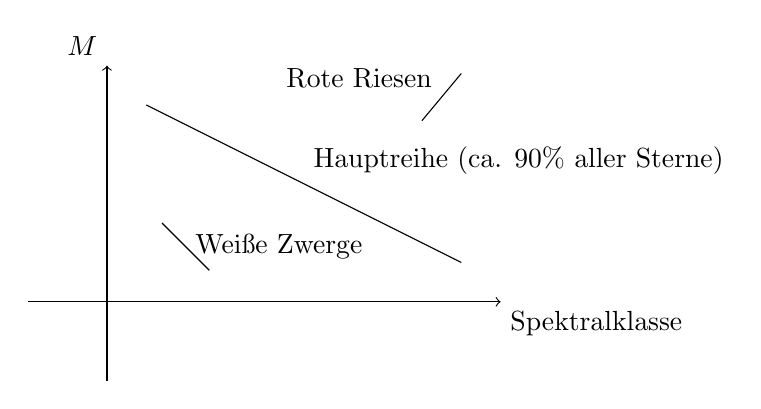
\begin{tikzpicture}
				\draw[->] (-1,0)--(5,0)node[below right]{Spektralklasse};
				\draw[->] (0,-1)--(0,3)node[above left]{$M$};
				\draw (0.5,2.5)--(4.5,0.5)node[midway,above right]{Hauptreihe (ca. $\SI{90}{\%}$ aller Sterne)};
				\draw (0.7,1)--(1.3,0.4)node[midway,right]{Weiße Zwerge};
				\draw (4,2.3)--(4.5,2.9)node[midway,above left]{Rote Riesen};
			\end{tikzpicture}
		\end{figure}
		Spektralklassen: $\underset{\SI{30000}{\K}-\SI{50000}{\K}}{O}$, $\underset{\SI{10000}{\K}-\SI{28000}{\K}}{B}$, $\underset{\SI{7500}{\K}-\SI{9750}{\K}}{A}$, $\underset{\SI{6000}{\K}-\SI{7350}{\K}}{F}$, $\underset{\SI{5000}{\K}-\SI{5900}{\K}}{G}$, $\underset{\SI{3500}{\K}-\SI{4890}{\K}}{K}$, $\underset{\SI{2000}{\K}-\SI{3350}{\K}}{M}$
		\begin{itemize}[label={}]
			\item Sonne: G2
			\item Sirius: A
			\item Betelgeuze: M
		\end{itemize}
	\item \textbf{Die Eigenschaften von Sternen auf der Hauptreihe werden im wesentlichen nur von einem Parameter bestimmt: der Masse $M$ dieser Sterne!}
	\item Riesen: Sterne der gleichen Spektralklasse wie Hauptreiensterne, aber mit viel größerer Leuchtkraft $L\Rightarrow R$ viel größer (vgl. $(\ast)$)
	\item Dieser Größeneffekt ist spektroskopisch zu erkennen: Schwerebeschleunigung eines Stern auf seiner Oberfläche: $g=\frac{\gamma M}{R^2}$ hat Einfluss auf die Breite von Spektrallinien des Sternes
		\begin{itemize}
			\item Zusammenhang zwischen Linienbreite und $R$ 
			\item $L$ mit Hilfe von $(\ast)$
		\end{itemize}
	\item Basierend auf der Schärfe von Spektrallinien teilt man die Sterne in die Leuchtkraftklassen ein:
		\begin{enumerate}[label={\Roman*:}]
			\item Überriesen
			\item Helle Riesen
			\item Riesen
			\item Unterriesen
			\item Zwerge
			\item Unterzwerge
		\end{enumerate}
	\item Kennt man die Entfernung $D$ (und $L$) kann man mit Hilfe der Liniebreite $g$ ermitteln
		\begin{itemize}
			\item Masse $M$
		\end{itemize}
	\item empirischer Zusammenhang zwischen $L$ und $M$ für Hauptreihensterne:
		\begin{equation*}
			\frac{L}{L_\odot}=\left(\frac{M}{M_\odot}\right)^\frac{7}{2} \qquad (\ast\ast)
		\end{equation*}
\end{itemize}
\subsection{Sternentwicklung}
\begin{itemize}
	\item Energiequelle: thermonukleare Reaktionen
	\item einfachster Prozess:
		\begin{equation*}
			4 {}^1\text{H} \to {}^4\text{He} + \SI{26.73}{Me\V}
		\end{equation*}
	\item zwei Haupt-Raktionsketten:
		\begin{enumerate}[label={(\roman*)}]
			\item pp-Kette ($T<\SI{15e6}{\K}$)
				\begin{align*}
					{}^1\text{H}+{}^1\text{H}&\to{}^2\text{H}+e^++\nu_e+\SI{0.42}{Me\V}\\
					{}^2\text{H}+{}^1\text{H}&\to{}^3\text{He}+\gamma+\SI{5.49}{Me\V}\\
					{}^3\text{He}+{}^3\text{He}&\to {}^4\text{He}+2{}^1\text{H}+\SI{12.85}{Me\V}
				\end{align*}
				Energieerzeugungsrate $~\propto T^4$
			\item CNO-Zyklus (Bethe-Weizsäcker):
				\begin{align*}
					{}^{12}\text{C}+{}^1\text{H}&\to {}^{13}\text{N}+\gamma \to {}^{13}\text{C}+e^+\nu+\gamma\\
					{}^{13}\text{C}+{}^1\text{H}&\to {}^{14}\text{N}+\gamma+\SI{7.55}{Me\V}\\
					{}^{14}\text{N}+{}^1\text{H}&\to {}^{15}\text{O}+p \to {}^{15}\text{N}+e^++\nu+\gamma+\SI{10.05}{Me\V}\\
					{}^{15}\text{N}+{}^1\text{H}&\to {}^{12}\text{C}+{}^4\text{He}
				\end{align*}
				Energieerzeugungsrate $\propto T^{20}$
		\end{enumerate}
	\item erzeugte Energie während des zentralen Wasserstoffbrennens:
		\begin{equation*}
			\underset{\text{"`main sequence"'}}{E_{MS}}=\num{0.1}Mc^2\cdot\underset{\underset{\text{Energieerzeugung}}{\text{Effizienz der}}}{\num{0.007}}
		\end{equation*}
		\begin{itemize}
			\item Lebensdauer $t_{MS}$ eines Sterns der Hauptreihe: $E_{MS}=L\cdot t_{MS}\Leftrightarrow t_{MS}=\frac{E_{MS}}{L}=\num{8e9}\cdot \frac{\frac{M}{M_\odot}}{\frac{L}{L_\odot}} \si{\year}\overset{(\ast\ast)}{=} \num{8e9}\left(\frac{M}{M_\odot}\right)^{-\frac{5}{2}}\si{\year}$\\
				Stern mit $M\approx 100 M_\odot: $ $t_\odot\propto \underset{\underset{\text{astronomischer Zeitskala}}{\text{kurz auf}}}{\num{1}-\SI{3}{M\year}}$
		\end{itemize}
	\item \textbf{Sternentwicklung nach der Hauptreihe} in Abhängigkeit von $M$:
		\begin{enumerate}[label={(\roman*)}]
			\item $M<\num{0.7}M_\odot$: Entwicklung unbekannt, da $t_{ns}>$ Alter des Universums (befinden sich noch auf der Hauptreihe)
			\item $M<\num{2.5}M_\odot$: Helumbrennen im Kern $\underset{\text{triple-$\alpha$}}{(3{}^4\text{He}\to{}^{12}\text{C})}$ setzt ein und verläuft explosiv ("`Helium-Flash"')
				\begin{itemize}
					\item stabile GG-Konfiguration mit erhöhtem Radius $R$ $\Rightarrow $ Roter Riese oder Überriese
						\begin{figure}[H]
							\centering
							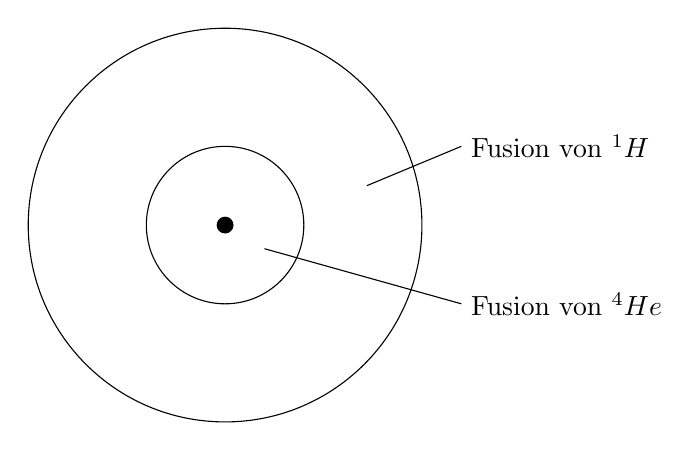
\begin{tikzpicture}
								\draw (0,0)circle(2.5 cm);
								\draw (0,0)circle(1 cm);
								\draw[fill=black] (0,0)circle(1 mm);
								\draw (0.5,-0.3)--(3,-1)node[right]{Fusion von ${}^4\text{He}$};
								\draw (1.8,0.5)--(3,1)node[right]{Fusion von ${}^1\text{H}$};
							\end{tikzpicture}
						\end{figure}
					\item[] Brennen in Form von Pulsen $\to$ Abstoßung der Hülle des Sternes $\Rightarrow$ Weißer Zwert ($M\sim \num{0.6}M_\odot$ und $R\sim\SI{5000}{k\m}$)
				\end{itemize}
			\item $\num{2.5}M_\odot < M < \num{8}M_\odot$:
				\begin{itemize}[label={$\cdot$}]
					\item Zentrale Helium-Brennzone + Fusion von ${}^1\text{H}$ in Schale
					\item Massenverlust durch Sternwind
						\begin{itemize}
							\item[$\Rightarrow$] Weißer Zwerg (falls $M_{final}<\num{1.4}M_\odot$)
						\end{itemize}
				\end{itemize}
			\item $M>8M_\odot$:
				\begin{itemize}[label={$\cdot$}]
					\item CNO-Zyklus und weitere Fusionen bis zur Erzeugung von $\text{Fe}$ im Kern
					\item Eisenkern kollabiert, falls $M_{final}>\num{1.4}M_\odot$
						\begin{itemize}
							\item[$\Rightarrow$] Supernova + Neutronenstern oder schwarzes Loch
						\end{itemize}
				\end{itemize}
		\end{enumerate}
\end{itemize}
